\documentclass[12pt,a4paper]{article}
\usepackage{pgf, tikz}
\usetikzlibrary{arrows, automata}
\usepackage[T1]{fontenc}
\usepackage[utf8]{inputenc}
\usepackage{lmodern}
\usepackage{tocloft}
\usepackage{graphicx}
\usepackage{amsmath,amsthm}
\usepackage[ampersand]{easylist}
\usepackage{blindtext}
\usepackage{enumitem}
\usepackage{polski}
\usepackage{listings}
\usepackage{thmtools}

\usepackage{float}

\usepackage{amssymb}
\newcommand{\symcom}[1]{\mathcal{#1}}
\newcommand{\powset}[1]{\mathcal{P}(#1)}
\newcommand{\dims}[1]{\text{dim }#1}
\newcommand{\fun}[3]{#1:#2 \rightarrow #3}
\newcommand{\Rn}[0]{\mathbb{R}^n}
\newcommand{\set}[1]{ \{#1\}}
\newcommand{\gemsym}[2]{\big<#1,	\ldots,#2\big>}

\newtheorem{twr}{Twierdzenie}[section]
\newtheorem{example}{Przykład}[section]
\newtheorem{definition}{Definicja}[section]

\title{Praca Magisterska}
\author{jbanaskiewicz.jb }
\date{February 2019}

\begin{document}
\maketitle

\section{Wstęp}
Pojęcie układów dynamicznych jest pojęciem pojawiającym się w matematyce w wielu odsłonach. Są one zwykle modelowane przez pewną funkcje $\fun{\varphi }{X\times T}{X}$, gdzie $X$ jest pewną przestrzenią a $T$ zbiorem czasów. Funkcja ta pozwala nam zobaczyć ewolucję punktu $x\in X$ w dowolnym czasie $t$ ze zbioru $T$. Zwykle wymagamy, żeby zbiór $T$ rozsądnie modelował czas czyli do $T$ powinno należeć $0$ oraz jeśli $t,s\in T $
to także $t+s\in T$. Funkcja ta powinna spełniać zależności:
\\(i)$\varphi(x,0) = x$
\\(ii)$\varphi(x,t+s) =\varphi(\varphi(x,t),s)$
\noindent
\\
Pierwsza własność mówi nam o tym, że przesunięcie puntu o czas $0$ da nam ten sam punkt. Druga natomiast mówi nam, że jeśli dany punkt przesuniemy w czasie $t$ a później o $s$ to dostaniemy to samo jakbyśmy przesunęli ten punkt w czasie $s+t$. Zwykle wymaga się dodatkowo aby nasz układ był ciągły w topologi produktowej $X\times T$. 
Jednymi z najbardziej rozpowszechnionych układów dynamicznych są układy pochodzące od równań różniczkowych zwyczajnych. Zakładając dostateczną regularność pola wektorowego oraz to, że rozwiązania nie wybucha w skończonym czasie można otrzymać układ dynamiczny $\varphi(x,t) = y(t)$, gdzie $y(t)$ jest rozwiązaniem danego równania różniczkowego spełniające $y(0)=x$. Spojrzenie w taki sposób na równania różniczkowe zwyczajne pozwala na badanie wielu ciekawych fenomenów dynamicznych jak punty stałe i ich stabilność, orbity okresowe, chaotyczne zachowania. Innym przypadkiem układów dynamicznych są układy pochodzące od iteracji odwzorowań. Wtedy zbiorem $T$ jest zbiór $\mathbb{N}$ a odwzorowanie $\varphi(x,n)$ jest równe $n$-tej iteracji odwzorowania. W każdym z tych przypadków definiuje się podstawowe pojęcia związanie z dynamiką takie jak orbita punktu czyli zbiór $o(x)=\{\varphi(x,t)|t\in T\}$ oraz zbiory nie zmienicze czyli takie, że orbita dowolnego punktu z tego zbioru zostaje także w tym zbiorze.
\\
W swojej pracy przedstawie układy dynamiczne pochodzące z dyskretnych struktur. Naszą przestrzenią $X$ będzie skończony zbiór sympleksów czyli kompleks symplicjalny. Jednakże rolę funkcji $\varphi$ będzie pełniła iteracja odwzorowania wielowartościowego czyli takiego, że $x\in X$ może przyjmować więcej niż jedną wartość. Odwzorowanie będzie to pochodziło od pewnej kombinatorycznej struktury na $X$, które będzie zwane dyskretnym polem wektorowym.
\\
\noindent
[Coś, że jest to naturalne gdy aproksymujemy pole wektorowe]
\\W dalszej części pracy przedstawie konstrukcje ciągłego pola wektorowego, którego to dynamika była by podobna do zadanego dyskretnego pola wektorowego. [Odnośnik do pracy z, której korzystam]
Podobieństwo to polega na porównywaniu grafów Conleya-Morse’a. Ich konstrukcja opiera się o indeks Conleya. Grafy Conleya-Morse’a. tak samo jak indeks Conlaya można sensownie zdefiniować dla układów pochodzących od równania różniczkowego jak i dyskretnych pól wektorowych.
\\
\noindent
Jeśli kompleks symplicjalny da się zanurzyć w przestrzeni $\mathbb{R}^2$ to równanie równikowe zwyczajne, które pochodzi od pewnego pola dyskretnego wektorowego na tym sympleksie powinno się być w stanie przedstawić w postaci portretu fazowego zawartego w $\mathbb{R}^2$. Jednak zaprezentowana konstrukcja zapisuje to równanie względem innych zmiennych niż standardowa baza $\mathbb{R}^2$ a liczba zmiennych w tym równaniu zależy nie wymiaru przestrzeni w, której to jest on zanurzony a liczbie wierzchołków tego sympleksu. W pracy tej proponuje rzutowanie tego równania w taki sposób by otrzymać wektorowe w $\mathbb{R}^2$. Wykorzystuje to rzutowanie do zrobienia wizualizacji portretu fazowego dla równania różniczkowego które pochodzi od dyskretnego pola wektorowego. Program do tego zadania napisałem w notebooku Mathematica, a portret fazowy rysuje za pomocą funkcji StreamPlot.
\\
\noindent
[Struktura pracy]



\section{Kompleksy symplicjalne}

\subsection{Afiniczna niezależność}
[charakterystyka otoczki wypukłej zbiorów skończonych]
\\
\noindent
Niech $v_0,\ldots,v_n\in\Rn$ kombinacja wypukłą tych wierzchołków będziemy nazywać wyrażenie postaci
$$\lambda_0v_0 + \dots + v_n\lambda v_n\text{, gdzie }\sum_{i=0}^n\lambda_i=1 \text{ oraz }\lambda_i\in[0,1]$$
Istnieje charakterystyka otoczki wypukłej skończonego zbioru $\set{v_0,\ldots,v_n}$, która mówi, że dowolny punkt z tej otoczki daje się przedstawić jako kombinacja wypukła punktów $v_0,\ldots, v_n$ oraz dowolna kombinacja wypukła tych punktów leży w otoczce. 
Jeśli każdy element z otoczki wypukłej zbioru $\set{v_0,\ldots,v_n}$ da się jednoznacznie zapisać za pomocą kombinacji wypukłej to punkty $v_1,\ldots ,v_n$ będziemy nazywać afiniczne niezależnymi.

\subsection{Kompleksy symplicjalne w $\Rn$}
Rozważmy zbiór punktów $v_0,\ldots,v_k\in\Rn$ i załóżmy, że są afiniczne niezależne. Wtedy otoczkę wypukłą punktów $v_0,\ldots,v_k$ oznaczmy $\gemsym{v_0}{v_k}$ i nazywamy ją $k$ wymiarowym sympleksem rozpiętym przez wierzchołki $v_0,\ldots,v_k$. Z definicji afinicznej niezależności każdy punkt $x\in\gemsym{v_0}{v_k}$ możemy jednoznacznie zapisać jako
$$x=\sum_{i=0}^{k}\lambda_{v_0}(x)v_i, \text{ gdzie } \sum_{i=0}^{k}t_{v_i}=1 \text{ oraz } \lambda_{v_i}(x)\in[0,1]$$
Funkcja $\fun{\lambda_{v_i}}{\gemsym{v0}{vk}}{[0,1]}$ zdefiniowana jako współczynnik przy $v_i$ w powyższej kombinacji jest nazywana współrzędną barycentryczną względem wierzchołka $v_i$. 
Ścianą sympleksu nazywamy sympleks, który rozpięty jest przez podciąg $v_{i_0},\ldots,v_{i_p}$, jeśli $p<k$ to ścianę tą nazywamy ścianą właściwą. 
\begin{definition}
Kompleksem symplicjalnym w $\Rn$ będziemy nazywali zbiór $\symcom{S}$ sympleksów spełniających warunki
\\(i)Dla każdego $s\in\symcom{S}$ jego ściany także należą do $\symcom{S}$ 
\\(ii)Dla każdego $s_1,s_2\in\symcom{S}$ część wspólna $s_1$ i $s_2$ jest ich wspólną ścianą.
\end{definition} 
\\W kolejnych sekcjach taki kompleks symplijalny będziemy nazywać geometrycznym kompleksem symplicjalnym by można go było odróżnić od abstrakcyjnego kompleksu symplicjalnego.
\noindent
Niech $\symcom{S}$ będzie kompleksem symplicjalnym.
Wymiarem kompleksu $\symcom{S}$ nazywa się maximum z wymiarów należących do nie go sympleksów. Bryłą $\symcom{S}$ nazywamy zbiór
$$|\symcom{S}|:=\bigcup_{s\in\symcom{S}}s$$
Poprzez $\symcom{S}_k$ będziemy oznaczać zbiór k wymiarowych sympleksów. W szczególności zbiór $\symcom{S}_0$ będzie zbiorem wierzchołków kompleksu symplicjalnego. Każdy punkt $x\in{|\symcom{S}|}$ daje należy do pewnego kompleksu symplicjalnego. Co więcej z definicji kompleksu symplicjalnego jeśli należy do dwóch różnych sympleksów to także musi leżeć w ich wspólnej ścianie. Co za tym jeśli zapiszemy $x$ współrzędnych barycentrycznym względem dwóch różnych sympleksów z $\symcom{S}$ do których on należy to muszą być one takie same.  Możemy więc zapisać x w postaci
$$
x=\sum_{v\in \symcom S _0}t_v(x) v\text{ gdzie}\sum_{v\in \symcom S_0}t_v(x) = 1\text{ oraz }t_v(x)\in[0,1]
$$
By przedstawić $x$ w takiej postaci należy najpierw znaleźć sympleks $\gemsym{v_0}{v_k}$ do którego $x$ należy i zapisać go w
współrzędnych barycentrycznych $\lambda_{v_i}(x)$ względem tego sympleksu. Potem wystarczy przyjąć za $t_{v_i})
(x)$ współrzędną $\lambda_{v_i}(x)$ a gdy $v\in\symcom S_0$ nie jest wierzchołkiem rozpinającym sympleks to kładziemy $t_v(x) =0$. Zauważmy, że powstały rozkład nie zależy od wyboru sympleksu do który wybraliśmy na początku procedury co wynika z obserwacji poczynionej powyżej. Podobnie jak w przypadku sympleksu funkcje $\fun{t_v}{|\symcom{S}|}{[0,1]}$ będziemy nazwali współrzędną barycentryczną względem wierzchołka $v$.



\subsection{Abstrakcyjne kompleksy}
\begin{definition}
Niech $X$ będzie dowolnym skończonym zbiorem zbiorem. Jeśli $\symcom{X}$ jest niepustym zbiorem podzbiorów X oraz dla każdego $s\in\symcom{X}$ wszystkie niepuste podzbiory $s$ należą do $\symcom{X}$ to $\symcom{X}$ będziemy nazywali abstrakcyjnym kompleksem symplicjalnym.
\end{definition}
\noindent
\\
Niech $\symcom{X}$ będzie abstrakcyjnym kompleksem symplicjalnym a $s,u$ jego elementami. Wymiarem sympleksu $s,u$ nazywamy liczbę $\dims{s}=|s|-1$. Jeśli $s\subset u$ to mówimy, że $s$ jest ścianą $u$, dodatkowo gdy $s \neq u$ to $s$ jest właściwą ścianą $u$. Wymiarem całego kompleksu symplicjalego będziemy nazywać maximum z wymiarów sympleksów które należą do tego kompleksu symplicjalnego. Jeśli $\mathcal{X}_1\subset \mathcal{X}$ jest także kompleksem symplicjalnym to $\mathcal{X}_1$ jest podkompleksem $\mathcal{X}$
\noindent

Zobaczmy, że dowolny geometryczny kompleks symplicjalny  $\symcom S$ można przedstawić jako abstrakcyjny kompleks symplicjalny.  Jako $X$ weźmiemy zbiór wierzchołków kompleksu $\symcom S _0$ i utworzymy zbiór
$$\symcom{X}_\symcom{S}=\set{s\cap\symcom{S}_0\in\X|s\in\Symcom {S}}$$
Zbiór ten jest abstrakcyjnym kompleksem symplijalnym nad X gdyż jeśli  $\set{v_0,\ldots,v_n}$ jest w $\symcom{X}_\symcom{S}$ to dowolna ściana tego sympleksu jest w $\symcom{S}$ więc przecinając ją ze zbiorem wierzchołków dostaniemy dowolny podzbiór zbioru $\set{v_0,\ldots,v_n}$. Dla danego sympleksu w $s\in S$ przez $\symcom_{X}_s$ będziemy oznaczali odpowiadający mu element w abstrakcyjnym kompleksie symplicjalnym czyli zbiór $s\cap\symcop S _0$

\noindent
\\
 Łatwo można zobaczyć, że pojęcia zdefiniowane powyżej dla abstrakcyjnego kompleksu symplijalngo pokryją się z analogicznymi pojęciami zdefiniowanego dla geometrycznego kompleksu symplijalnego. Wymiary sympleksów w geometrycznym i utworzonym od niego abstrakcyjnym kompleksie są takie same. Dodatkowo $s_1$ jest ścianą (ścianą właściwą) $s_2$ w geometrycznym kompleksie symplijalnym to $\symcop{X}_{s_1}$ jest ścianą (ścianą właściwą) sympleksu $\symcop{X}_{s_2}$

\subsection{Geometryczna realizacja kompleksów}
Zadajmy teraz pytanie czy dla dowolnego abstrakcyjnego kompleksu symplicjalnego jesteśmy wstanie znaleźć jego geometryczny odpowiednik. Najpierw jednak zdefiniujemy przez co będziemy rozumieć przez geometryczną realizacje kompleksu symplijcalnego. Rozważmy abstrakcyjny kompleks symplicjalny $\symcom X$ oraz funkcje $\fun{\eta}{\symcom{X}_0}{\Rn}$. Przyjmiemy konwencje, że dla sympleksu $\set{v_0,\ldots,v_k}$ przez $\eta(\set{v_0,\ldots,v_k})$ będziemy oznaczać otoczkę wypukłą punktów $\eta(v_0),\ldots,\eta(v_k)$.
\begin{definition}
Dla kompleksu symplicjalego $\symcom{X}$ jego geometryczną realizacją będziemy nazywali funkcje $\fun{\eta}{\symcom{X}_0}{\Rn}$ która dla każdego $s,u\in\symcom{X}$ spełnia 
\\(i) $\eta(v_0),\ldots,\eta(v_k)$ są afiniczne nie zależne gdy $\set{v_0,\ldots,v_k}\in\symcom{X}$
\\(ii) $\eta(s\cap v) = \eta(s)\cap\eta(u)$
 \end{definition}
\\
[Pokazać, że spełnia to załorzenia abstrakcyjnego kompleksu symplicjalnego ]
\noindent
[Przykład, że geometryczna realizacja nie jest jednoznaczna]
\\Niech $\symcop{X}_0=\set{v_0,\ldots,v_n}$ i ustalmy $\eta_j(v_i) = \delta_{ij} $, gdzie  $\delta_{ij}$ jest deltą Kroneckera i przyjmijmy $\eta(v_i) =(\eta_0(v_i),\ldots ,\eta_n(v_i))$. Zaobserwujmy, że dla dowolnego kompleksu symplicjalnego $\symcop{X}$, dla którego zbiorem wierzchołków jest zbiór jest zbiór $\symcom{X}_0$ tak zdefiniowana $\eta$ jest geometryczną realizacją tego sympleksu. Ponieważ $\eta(v_0),\ldots,\eta(v_n)$ tworzy bazę standardową w przestrzeni przestrzeni $\mathbb{R}^{n+1}$ to dowolny układ z $\eta(v_{i_0}),\ldots,\eta(v_{i_p})$ jest liniowo niezależny. Łatwo zauważyć, że implikuje to, że układ $\eta(v_{i_0}),\ldots,\eta(v_{i_p})$ jest także afiniczne niezależny co pociąga za sobą, że punkt $(i)$ jest spełniony. By pokazać $(ii)$ ustalmy $x\in\eta({s\cap u})$ gdzie $s,u$ są sympleksami z $\symcom{X}$ wtedy $x$ mogę przedstawić jako kombinację wypukłą $\sum_{v\in s\cap u}\lambda_i\eta(v)$, więc dopisując zera mogę ją zapisać jako kombinacja wypukła wierzchołków z $s$ oraz $u$. Jeśli $x\in\eta(s)$ i $x\in\eta(u)$ to zapisując $x$ jako kombinacje wypukłe względem tych zbiorów i korzystając z tego, że  $\eta(v_0),\ldots,\eta(v_n)$ jest układem liniowo nie zależnym to współczynniki przy wyrazach $\eta(v)$ są zerowe jeśli $v$ nie należy do $s\cap u  $ i co za tym idzie $x\in\eta(u\cap v)$ co pokazuje (ii). Taką konstrukcję dla kompleksu $\symcom{X}$ będziemy oznaczali  
\\
 \\
 \noindent
 Zaobserwujmy, że jeśli $\symcom{S}$ jest geometrycznym kompleksem to konstrukcja ta zwykle umieszcza kompleks $\symcom{X}_{\symcom{S}}$ w przestrzeni więcej wymiarowej niż pierwotnie leżał kompleks symplicjalny $\symcom {S}$, ponieważ każdemu z wierzchołkowi przypisuje oddzielny wymiar. Warto na tę konstrukcje spojrzeć przy pomocy współrzędnych barycentrycznych. Jeśli $v_0,\ldots,v_n$  są wierzchołkami $\symcom{S}$ i $x\in|\symcom{S}|$ to odpowiadającym mu punktem w powyższej konstrukcji będzie punkt $(t_{v_0}(x),\ldots,t_{v_n}(x))$  więc każda barycentryczna współrzędna została potraktowana jako osobna współrzędna w $\mathbb{R}^{n+1}$
\subsection{Topologia w abstrakcyjnych kompleksach}

Niech $\mathcal{X}$ będzie abstrakcyjnym kompleksem symplicjalnym i $s\in X$. Domknięciem sympleksu $s$ nazywamy zbiór 
$$\text{cl }s=\{u\in \mathcal{X}|u\subset s \}$$
 Jest to zbiór składający się z wszystkich ścian $s$. Jeśli $\mathcal{R}$ jest podzbiorem abstrakcyjnego kompleksu $\mathcal{X}$ to domknięciem $\mathcal{R}$ będziemy nazywać sumę domknięć wszystkich sympleksów do niego należących i oznaczamy $\text{cl }\mathcal{R}$. Równoważnie można powiedzieć, że jest to najmniejszy podkompleks $\mathcal{X}$, który zawiera sympleksy z $\mathcal{R}$.  Jeśli spełniona jest równość $\text{cl }\mathcal{R} =\mathcal{R}$ to zbiór $\mathcal{R}$ będziemy nazywali zbiorem domkniętym. Zauważmy, że zbiór domkniętych zbiorów spełnia standardowe aksjomaty topologiczne. Domknięcie zbioru pustego $\emptyset$ jest zbiorem pustym a domknięcie zbioru $\mathcal{X}$ jest zbiorem $\mathcal{X}$ czyli zbiór pusty i cała przestrzeń jest domknięta. Jeśli $\mathcal{}$ $\mathcal{R}_1,\mathcal{R_2}$ są domknięte to ich suma i iloczyn także. Ponieważ zbiór $\mathcal{X}$ jest skończony implikuje to, że dowolne iloczyn dowolnej rodziny zbiorów domkniętych jest domknięty. Pokazuje to, że zbiór ten stanowi topologie
\\[Przykład kompleksu ze skończoną topologią]
\subsection{Grupy homologii}

[Dopisać skrajne przypadki]
Niech $\mathcal{X}$ będzie abstrakcyjnym kompleksem symplicjalnym. Grupą $n$-wymiarowych Łańcuchów nad $\mathbb{Z}_2$ nazywamy zbiór
$$C_n(\mathcal{X},\mathbb{Z}_2):=\{\fun{\sigma}{\mathcal{X}_n}{\mathbb{Z}_2 }\}$$
wraz z operacją dodawania daną wzorem $(\sigma_1+\sigma_2)(x):=(\sigma_1(x)+\sigma_2(x))\text{ mod } 2$.
Zauważmy, że grupa ta stanowi przestrzeń wektorową z bazą złożoną z funkcji
$$
\sigma_s(x)=
\begin{cases} 
1\text{ gdy }s=x
\\0\text{ wpp}
\end{cases}
\text{ dla } s\in\mathcal{X}_n
$$ 
Dla uproszczenia notacji funkcje te utożsamimy z  $n$-wymiarowymi sympleksami z kompleksu. Korzystając z ten konwencji każdy łańcuch $c\in C_n(\mathcal{X},\mathbb{Z}_2)$ można zapisać w postaci
$$c=\sum_{s\in\mathcal{X}_n}\alpha_s s  \text{ gdzie }\alpha_s\in \mathbb{Z}_2$$
Odwzorowanie $\fun{\partial_n}{C_n(\mathcal{X},\mathbb{Z}_2)}{C_{n-1}(\mathcal{X},\mathbb{Z}_2)}$ dane dla bazowych elementów wzorem
$$\partial_n s = \sum_{v\in s}s\setminus \{v\}$$
i liniowo rozszerzone na całe $C_n(\mathcal{X},\mathbb{Z_2})$ jest nazywane operatorem brzegu. Intuicyjnie dla danego $n$-wymiarowego sympleksu $s$ zwraca on nam łańcuch złożony z jego $(n-1)$-wymiarowych ścian.
Operator ten spełnia równość $\partial_{n-1}\partial_{n}=0$. Dla $s\in\mathcal{X}_n$ mamy
$$\partial_n\partial_{n-1}(s)=\sum_{v_1\in s}\;\sum_{v_2\in s\setminus \{v_1\}}s\setminus\{v_1,v_2\} $$
Wyrazami tej sumy są $(n-2)$-wymiarowe ściany postaci $s\setminus\{v_a,v_b\}$, gdzie $v_a,v_b\in s$ i $v_a\not =v_b$. Każdą z takich ścian występuje w powyższej sumie dwa razy co powoduje, że współczynnik przy tej ścianie wynosi zero.

\\Grupą cykli nazywamy grupę $Z_n(\mathcal{X},\mathbb{Z}^2)= \text{ker }\partial_n$ a grupą brzegów grupę $B_n(\mathcal{X},\mathbb{Z}_2) = \text{im } \partial_{n+1}$. Ponieważ $\partial_{n-1}\partial_n = 0$ to grupa brzegów stanowi podgrupę grupy cykli. Możemy zatem utworzyć grupę ilorazową 

$$H_n(\mathcal{X},\mathbb{Z}^2):= Z_n(\mathcal{X},\mathbb{Z}^2)/B_n(\mathcal{X},\mathbb{Z}_2) $$
Grupę tą nazywamy n-wymiarową grupą homologi. Dla geometrycznego kompleksu symplicjalnego $\mathcal{S}$ przez $H_n(\mathcal{S},\mathbb{Z}^2)$ będziemy oznaczać grupy homologi kompleksu $\mathcal{X}_\mathcal{S}$. Zaskakującym faktem jest to, że dla dwóch geometrycznych kompleksów symplicjalnych $\mathcal{S}_1,\mathcal{S}_2$ jeśli realizują one te same bryły czyli $|\mathcal{S}_1|=|\mathcal{S}_2|$ to grupy homologi $H_n(\mathcal{S}_1,\mathbb{Z}^2)$ i $H_n(\mathcal{S}_2,\mathbb{Z}^2)$ są izomorficzne dla każdego $n\in \mathbb{N}$. Co więcej jeśli bryły $|\mathcal{S}_1|$ i $|\mathcal{S}_2| $ są homeomorficzne to ich grupy homologi także są takie same.
\\Jeśli $\mathcal{A}$ stanowi podkompleksem $\mathcal{X}$ to $C_n(\mathcal{A},\mathbb{Z}_2) $ stanowi podgrupę $C_n(\mathcal{X},\mathbb{Z}_2) $. Zdefiniujmy grupę ilorazową
$$C_n(\mathcal{X}/\mathcal{A},\mathbb{Z}_2):=C_n(\mathcal{X},\mathbb{Z}_2)/C_n(\mathcal{A},\mathbb{Z}_2)$$
, którą nazywamy relatywną grupą $n$-wymiarowych łańcuchów. Dzięki temu, że $\mathcal{A}$ jest podkompleksem $\mathcal{X}$ to wzór 
$$\widetilde{\partial_n} [s] = [\partial_n s]\text{ gdzie }[s]\in C_n(\mathcal{X}/\mathcal{A},\mathbb{Z}_2) $$
Zadaje poprawną funkcje $\fun{\widetilde{\partial_n}}{C_n(\mathcal{X}/\mathcal{A},\mathbb{Z}_2)} {C_{n-1}(\mathcal{X}/\mathcal{A},\mathbb{Z}_2)}$ nazywaną relatywnym operatorem brzegu. W tym przypadku także zachodzi równość $\widetilde{\partial_n} \widetilde{\partial_{n-1}}=0$ więc  poważając konstrukcje grup homologi definiujemy odpowiednio relatywną grupę cykli $Z_n(\mathcal{X}/\mathcal{A},\mathbb{Z}_2):=\text{ker }\widetilde{\partial_n}$ oraz relatywną grupę brzegów  $B_n(\mathcal{X}/\mathcal{A},\mathbb{Z}_2):=\text{im }\widetilde{\partial_n}$. Relatywną grupą homomologi będziemy nazywać grupę
$$H_n(\mathcal{X}/\mathcal{A},\mathbb{Z}^2):= Z_n(\mathcal{X}/\mathcal{A},\mathbb{Z}^2)/B_n(\mathcal{X}/\mathcal{A},\mathbb{Z}_2) $$
\section{Dyskretne pola wektorowe}
\noindent
W tej sekcji zdefiniujemy dyskretne pola wektorowe na $\symcom{X}$. Jest to rozszerzenie teorii Formana
\begin{definition}
Niech $\symcom {X}$ będzie abstrakcyjnym kompleksem symplicjalnym. Podział $\symcom{V}$ zbioru $\symcom{X}$  będziemy nazywać Dyskretnym polem wektorowym gdy każdego $v\in\symcom{V}$ zachodzi jeden z poniższych warunków.
\\(i)$v=\set{s}$, gdzie $s\in\symcom{X}$
\\(ii)$v=\set{s_1,s_2}$,  gdzie $s_1,s_2\in\symcom{X}$ oraz $s_1\subset s_2$ i $\dims {s_1}  + 1 =\dims{s_2} $


\end{definition}
\noindent
Niech $\symcom{V}$ będzie polem wektorowym. Każdy z wektorów jest singletonem lub dubletonem. W przypadku singletona początkiem i końcem wektora będziemy nazywać sympleks zawarty w tym wektorze. Natomiast gdy wektor jest dwu elementowy to początkiem tego wektora będziemy nazywali sympleks o mniejszej liczności natomiast końcem sympleks o większej. Dla danego wektora $v\in\symcom V$ przez $v^-$ oznaczamy początek wektora $v$ a przez $v^+$ jego koniec. 

\section{Index Conley'a dla ciągłych układów dynamicznych}
\begin{definition}
Niech $X$ będzie domkniętym podzbiorem $\Rn$ .Ciągłą funkcję $\fun{\varphi}{X}{\mathbb{R}}$ będziemy nazywali potokiem gdy dla wszystkich $x\in X$ i $t,s\in \Rn$ spełnia warunki
\\(i) $\varphi(x,0)=x$
\\(ii) $\varphi(x,s+t)=\varphi(\varphi(x,s),t)$
\end{definition}

\\Niech $\varphi$ będzie układem dynamicznym. Orbitą $x\in X$ będziemy nazywali zbiór $o(x):=\{\varphi(x,t)|t\in\mathbb{R}\}$.Analogicznie zbiór $o^+(x):=\{\varphi(x,t)|t\in [0,+\infty]\}$ nazywamy orbitą dodatnią punktu $x$ a zbiór $o(x)^-(x):=\{\varphi(x,t)|t\in[-\infty,0]\}$ orbitą ujemną punktu $x$. Zbiór $S$ będziemy nazywali zbiorem niezmieniczym jeśli dla wszystkich $x\in S$ orbita $x$ zawiera się w $S$. Zauważmy, że suma i iloczyn mnogościowy dwóch zbiorów niezmieniczych jest także zbiorem niezmnieniczym. Jeśli $N\subset X$ to częścią niezmieniczą $N$ nazywamy zbiór
$$\text{inv}(N):=\{x\in N | o(x)\subset N\}$$
Jest to największy zbiór niezmieniczy, który zawiera się w $N$. Przypuśmy, że $x\in \text{inv}(N) $ nie jest niezmieniczy. Będzie istnieć wtedy $x$ w niezmieniczej części zbioru $N$ dla którego $y=\varphi(x,t_1)\not\in\text{inv}(N)$. Więc $o(y)\not\subset{N}$ czyli po pewnym czasie $t_2$,punkt $y$ opuści zbiór $N$. Wtedy jednak $\varphi(x,t_1+t_2)=\varphi(y,t_2)\not\in N$ co jest sprzeczne z tym że, $x$ był w niezmieniczej części zbioru $N$ co pokazuje, że $\text{inv}(N)$ jest zbiorem niezmieniczym. Zobaczmy także, że dowolny zbiór niezmieniczy zawarty w $N$ musi zawierać się w jego części niezmieniczej.
\\Jeśli zwarty zbiór $N$ spełnia zależność 
$$\text{inv}(N)\subset \text{int}N$$
to jest on nazywany otoczeniem izolującym. Zbiór niezmieniczy $S$ będziemy nazywali izolowanym zbiorem niezmnieczym jeśli isntnieje otoczenie izolujące $N$ takie, że $\text{inv}(N)=S$. Łatwo zaobserwować, że dowolny zbiór niezmieczy, który zawiera się w izolowanym zbiorze niezmieniczym także będzie izolowany.
Dla $x\in X$ zbiory

$$\omega(x):=\bigcup_{t>0}\text{cl}( o^{+}(\varphi(x,t)))$$
$$\alpha(x):=\bigcup_{t<0}\text{cl}( o^{-}(\varphi(x,t)))$$
Będziemy nazywali odpowiednio zbiorami omega i alfa granicznymi.
\\Rozważmy izolowany zbiór niezmieniczy $S$. Niech $\mathcal{M}$ będzie kolekcją izolowanych zwartych zbiorów niezmieniczych zawierających się w $S$. Niech $<$ będzie ostrym częściowym porządkiem. Jeśli dla każdego $x\in S$ spełniony jest jeden z warunków
\\(i)$x$ leży w pewnym zbiorze niezmieniczym $M\in\mathcal{M}$ 
\\(ii)Jeśli $\omega(x)\subset M_1\in \mathcal{M}$ i $\alpha(x)\subset M_2\in\mathcal{M}$ to $M_1<M_2$
Wtedy poset $(\mathcal{M},<)$ będziemy nazywać rozkładem Morsa zbioru $S$.

\\ Jeśli znamy dynamikę to naturalną definicją relacji $<$ jest przyjęcie, że $M_1<M_2$ wtw. gdy istnieje $x\in S$ taki, że $\omega(x)\subset M_1\in \mathcal{M}$ i $\alpha(x)\subset M_2\in\mathcal{M}$. Może się jednak zdarzyć taka definicja relacji nie będzie relacją ostrą relacją częściowego porządku. Wtedy na zbiorze $\mathcal{M}$ nie można dokonać rozkładu Morsa.
\\
\begin{figure}[H]
    \centering
   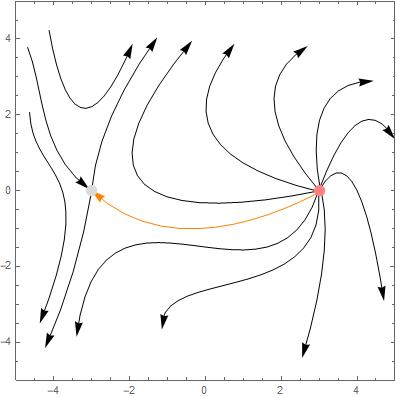
\includegraphics[width=0.55\textwidth]
   {IndexConley'a1.jpg}
    \caption{Układ dynamiczny z punktem odpychającym po prawej stronie i siodłem po lewej}
    \label{rys:index1}
   
\end{figure}
\\
\\
\begin{example}
Na rysunku \ref{rys:index1} widać układ dynamiczny w którym znajduje się zbiór niezmieniczy złożony z różowego punktu po lewej stronie, szarego punktu po prawej stronie i pomarańczowej trajektorii, która je łączy. Łatwo zauważyć, że jest to zbiór niezmieniczy izolowany ponieważ w jego otoczeniu nie ma żadnych innych zbiorów niezmieniczych. Same punkty także są izolowane. Przykładowe zbiory izolujące możemy zobaczyć na rysunku \ref{rys:index2}. Pomarańczowa trajektoria bez różowego i szarego punktu stanowi zbiór niezmieniczy ale nie jest on zbiorem izolowanym ponieważ niezmienicza część każdego zwartego otoczenia tej trajektorii zawiera dodatkowo różowy i szary punkt. 
\end{example}
\\
\\
\begin{figure}[H]
    \centering
   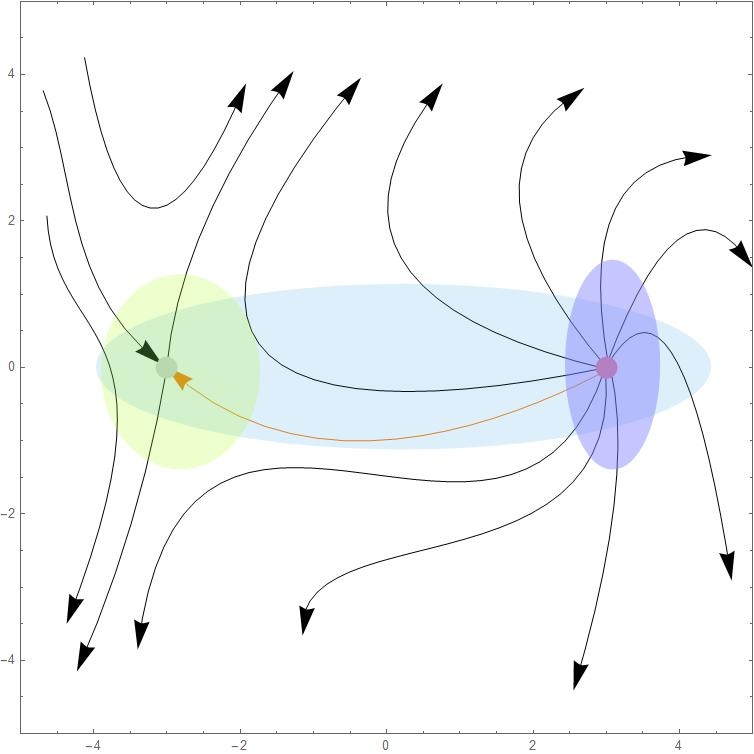
\includegraphics[width=0.5\textwidth]
   {IndexConley'a1Izolacje.jpg}
    \caption{Przykładowe otoczenia izolujące dla zbiorów niezmieniczych}
    \label{rys:index2}
\end{figure}
\\
\\
\\Niech $S$ będzie izolowanym zbiorem niezmieniczym. Para $(P_1,P_2)$ zwartych zbiorów takich $P_2\subset P_1$ nazywamy parą indeksową gdy zachodzą warunki
\\(i)$\text{inv}(\text{cl}(P_1\setminus P_2))=S$ oraz $N\setminus L$ jest otoczeniem $S$  
\\(ii)Jeśli $x\in P_2$ i trajektoria $\varphi(x,[0,t])$ zawiera się w $P_1$ to trajektoria $\varphi(x,[0,t])$ zawiera się także $P_2$ ($P_2$ jest pozytywnie niezmieniczy w $P_1$)
\\(iii)Jeśli dla $x\in P_1$ i pewnego $t_0>0$ zachodzi $\varphi(x,t_0)\not\in P_1$ wtedy istnieje $t_1\in[0,t_0]$ takie, że $\varphi(x,t)\in P_2$ ($P_2$ jest zbiorem wyjścia dla $P_1$)
\\
Jeśli $(P_1 ,P_2)$ jest parą indeksową to możemy utworzyć przestrzeń topologiczną z wyróżnionym punktem przez konstrukcje
\begin{enumerate}
\item Rozważyć topologie $\mathcal{T}_1$ indukowaną przez zbiór $P_1$ w $X$.
\item Z topologi $\mathcal{T}_1$ utworzyć topologie ilorazową $\mathcal{T}_2$ powstałą przez relacje, która utożsamia punkty ze zbioru $P_2$.
\item W topologi $\mathcal{T}_2$ wyróżnić punkt powstały z utożsamienia punktów zbioru $P_2$ .
\end{enumerate}
 Indeksem Conley'a nazywamy klasę homotopii powstałej z tej konstrukcji topologi. Pokazuje się, że ta klasa jest taka dla wszystkich par indeksowych.
 Ponieważ klasa homotopii jest ciężka do algorytmicznego policzenia to definiuje się homologiczny indeks Conley'a, który to jest niezmienikem klasy homotopii. W pracy ograniczymy definicji homotopijnego indeksu Conley'a dla par $(P_1,P_2)$ spełniających
\\ (i) Istnieje kompleks $\mathcal{S}_1 $ i jego podkompleks $\mathcal{S}_2$, których bryły stanową tą parę czyli $P_1=|\mathcal{S}_1|$ oraz $P_2=|\mathcal{S}_2|$
\noindent
\\(ii) Istnieje $U$ otoczenie $P_2$ w $P_1$, dla którego $P_2$ jest retraktem deformacyjnym $U$ 
\\Wtedy homotopijnym indexem Conley'a nazywamy kolekcje relatywnych grup homotopii $H(\mathcal{S}_1/\mathcal{S}_2,\mathbb{Z}_2)$.


\begin{enumerate}
\end{enumerate}
\begin{enumerate}
\end{enumerate}

\section{Pola wektorowe na kompleksach symplijalnych}
\subsection{Rzutowanie pól wektorowych}
 Niech $\symcom{S}$ będzie geometrycznym kompleksem symplicjalnym, oraz niech $v_1,\ldots,v_n$ będą wierzchołkami z kompleksu $\symcom{S}$.Będziemy rozważać pole wektorowe $y'(t) = f(y(t))$ dla którego zbiór $W=\set{(t_{v_1}(x),\ldots,t_{v_n}(x)|x\in |\symcom{S}|)}$ jest zbiorem niezmieniczym dla tego równania .Jest to warunek konieczny na to aby równanie równikowe zadane dla współrzędnych barycentrycznych mogło reprezentować pewne dyskretne pole wektorowe. Jeśli zbiór $W$ nie jest zbiorem niezmieniczym musi istnieć punkt w bryle tego kompleksu symplicjalego taki, że jego współrzędne barycentryczne po pewnym czasie przestaną sumować się do 1 więc przestanie reprezentować punkt w bryle kompleksu symplicjalnego.Oznacza to, że jeśli trajektoria $y(t)\in W$ dla wszystkich $t$ to musi ona spełniać równanie $y_1(t)+\ldots+y_n(t)=1$ dla wszystkich $t$. Po zróżniczkowaniu tego wyrażania względem $t$ dostajemy ${y'}_1(t)+\ldots+{y'}_n(t)=0$ i podstawiając ${y'}_i(t)=f_i(y(t))$ mamy
$$f_0(y(t))+\ldots+f_n(y(t))=0$$

\\
Zobaczmy także, że jeśli $y\in W$ oraz $y=(t_{v_1}(x),\ldots,t_{v_n}(x)$ dla $x\in|\symcom{S}|$ to musi istnieć sympleks $s\in \symcom{S}$ taki, że dla wszystkich wierzchołków $v_i$ które nie leżą w $s$ wartość pola wektorowego $f_i(y)$ musi wynosić $0$. Gdyby taki sympleks nie istniał to pole wektorowe w punkcie $y$ wskazywało by na zewnątrz zbioru $W$ i musiał by on opuścić ten zbiór.

\\
Zajmiemy się teraz problemem rzutowania pola wektorowego $f$ zapisanego w współrzędnych barycentrycznych kompleksu symplicjalnego $\symcom{S}$ na pole wektorowe, które jest zdefiniowane na bryle kompleksu symplicjalnego. Dla prostoty rozważmy nasze rozważania do kompleksu, który jest zanurzony w przestrzeni $\mathbb{R}^2$. Niech $\gamma(t)=(\gamma_1(t),\gamma_2(t))\subset\mathbb{R}^2$ będzie krzywą taką, że jej współrzędne barycentryczne spełniają równanie równanie różniczkowe zadane przez funkcje $f$. Mamy zatem 
$$
\begin{cases} 
\frac{d}{dt}[{t}_{v_1}(\gamma(t))] = f_1({t}_{v_1}(\gamma(t)),\ldots,{t}_{v_n}(\gamma(t)))
\\ \vdots  
\\ \frac{d}{dt}[{t}_{v_n}(\gamma(t))] = f_n({t}_{v_1}(\gamma(t)),\ldots,{t}_{v_n}(\gamma(t)))
\end{cases}
$$
Zgodnie z naszymi wcześniejszymi rozważaniami dla danego $\gamma(t_0)\in|\symcop{S}|$ możemy znaleźć taki sympleks $s \in\symcom{S}$ rozpięty na wierzchołkach $v_a,v_b,v_c$ taki, że dla wszystkich barycentrycznych współrzędnych z poza tego sympleksu $f({t}_{v_1}(\gamma(t_0)),\ldots,{t}_{v_n}(\gamma(t_0)))$ wynosi 0.
Pomijając te równania dostajemy układ.
$$
\begin{cases} 
\frac{d}{dt}[{t}_{v_a}(\gamma(t))] = f_a({t}_{v_1}(\gamma(t_0)),\ldots,{t}_{v_n}(\gamma(t_0)))
\\ \frac{d}{dt}[{t}_{v_b}(\gamma(t))] = f_b({t}_{v_1}(\gamma(t_0)),\ldots,{t}_{v_n}(\gamma(t_0)))
\\ \frac{d}{dt}[{t}_{v_c}(\gamma(t))] = f_b({t}_{v_1}(\gamma(t_0)),\ldots,{t}_{v_n}(\gamma(t_0)))
\end{cases}
$$
Korzystając z reguły łańcuchowej dostajemy układ.
$$
\begin{cases} 
\frac{d}{dx}{t}_{v_a}|_{(\gamma(t_0))} \frac{d}{dt}(\gamma_1(t_0)) +\frac{d}{dy}{t}_{v_a}|_{(\gamma(t_0))} \frac{d}{dt}(\gamma_2(t_0))
= f_a({t}_{v_1}(\gamma(t_0)),\ldots,{t}_{v_n}(\gamma(t_0)))
\\ 
\frac{d}{dx}{t}_{v_b}|_{(\gamma(t_0))} \frac{d}{dt}(\gamma_1(t_0)) +\frac{d}{dy}{t}_{v_b}|_{(\gamma(t_0))} \frac{d}{dt}(\gamma_2(t_0))
= f_b({t}_{v_1}(\gamma(t_0)),\ldots,{t}_{v_n}(\gamma(t_0)))
\\ \frac{d}{dx}{t}_{v_c}|_{(\gamma(t_0))} \frac{d}{dt}(\gamma_1(t_0)) +\frac{d}{dy}{t}_{v_c}|_{(\gamma(t_0))} \frac{d}{dt}(\gamma_2(t_0))
= f_c({t}_{v_1}(\gamma(t_0)),\ldots,{t}_{v_n}(\gamma(t_0)))
\end{cases}
$$
Zobaczmy, że jedno z tych równań jest redundantne.[Czemu] 
\\Zapisując dwa pierwsze równania w postaci macierzowej dostajemy równanie
 t $$
\begin{pmatrix} 
\frac{d}{dx}{t}_{v_a}|_{(\gamma(t_a))} & \frac{d}{dy}{t}_{v_a}|_{(\gamma(t_0))} \\
\frac{d}{dx}{t}_{v_b}|_{(\gamma(t_a))} & \frac{d}{dy}{t}_{v_b}|_{(\gamma(t_0))}
\end{pmatrix}
\,
\begin{pmatrix} 
\frac{d}{dt}(\gamma_1(t_0))  \\
\frac{d}{dt}(\gamma_2(t_0))
\end{pmatrix}
\,
=
\,
\begin{pmatrix} 
f_a({t}_{v_1}(\gamma(t_0)),\ldots,{t}_{v_n}(\gamma(t_0))) \\
f_b({t}_{v_1}(\gamma(t_0)),\ldots,{t}_{v_n}(\gamma(t_0)))
\end{pmatrix}
$$
Widzimy teraz, że jeśli potrafiliśmy byśmy wyznaczyć pochodne cząstkowe dla funkcji $t_{v_i}$ to odwracając macierz byli byśmy w stanie policzyć pole wektorowe, które zadaje krzywą $\gamma$. Ograniczę się teraz do wyznaczania tych pochodnych w przypadku dwóch sympleksów ponieważ tylko te przypadki realizuje w programie.
\\Przypuśmy, że $v_a=(1,0),v_b=(0,1),v_c=(0,0)$, jeśli punkt $(x,y)\in\big{<}(0,0),(1,0),(0,1)\big{>}$ to przedstawiając go w postaci kombinacji wypukłej tego wierzchołka otrzymamy
$$
(x,y) = x(1,0)+y(0,1)+(1-x-y)(0,0)
$$
Zatem współrzędne barycentryczne są dane wzorami  
\\$t_{(1,0)}(x,y)=x$
\\$t_{(0,1)}(x,y)=y$
\\$t_{(0,0)}(x,y)=(1-x-y)$
\\
Różniczkując dostajemy równość
$$
\begin{pmatrix} 
\frac{d}{dx}{t}_{(1,0)}|_{(\gamma(t_a))} & \frac{d}{dy}{t}_{(1,0)}|_{(\gamma(t_0))} \\
\frac{d}{dx}{t}_{(0,1)}|_{(\gamma(t_a))} & \frac{d}{dy}{t}_{(0,1)}|_{(\gamma(t_0))}
\,
\end{pmatrix}
=
\,
\begin{pmatrix} 
1 & 0 \\
0 & 1
\,
\end{pmatrix}
$$

Zatem mamy równanie
$$
\begin{pmatrix} 
\frac{d}{dt}(\gamma_1(t_0))  \\
\frac{d}{dt}(\gamma_2(t_0))
\end{pmatrix}
\,
=
\,
\begin{pmatrix} 
f_a({t}_{v_1}(\gamma(t_0)),\ldots,{t}_{v_n}(\gamma(t_0))) \\
f_b({t}_{v_1}(\gamma(t_0)),\ldots,{t}_{v_n}(\gamma(t_0)))
\end{pmatrix}
$$
Zatem w tym przypadku dostaliśmy wzór na pole wektorowe zrzutowane na $\mathbb{R}^2$.
\\
Przeprowadzając analogiczne rozumowanie, jeśli $v_a=(-1,0),v_b=(0,-1),v_c=(0,0)$ to dostaniemy wzór.
$$
\begin{pmatrix} 
\frac{d}{dt}(\gamma_1(t_0))  \\
\frac{d}{dt}(\gamma_2(t_0))
\end{pmatrix}
\,
=
\,
\begin{pmatrix} 
-f_a({t}_{v_1}(\gamma(t_0)),\ldots,{t}_{v_n}(\gamma(t_0))) \\
-f_b({t}_{v_1}(\gamma(t_0)),\ldots,{t}_{v_n}(\gamma(t_0)))
\end{pmatrix}
$$


Dodatkowo zauważmy jeśli przesuniemy wszystkie o punkty rozpinające sympleks o ten sam wektor to wzory na zrzutowone pole pozostaną takie same.
\subsection{Nie mam pomysłu na nazwe}
Niech $\symcop{S}$ będzie geometrycznym kompleksem symplicjalnym. Rozważmy dyskretne pole wektorowe $\symcop{V}$ na abstrakcyjnym kompleksie $\symcop{X}_{\symcop{S}}$. Przedstawimy teraz konstrukcje pola wektorowego, dla współrzędnych barycetrycznych, której graf [Kogo] jest taki sam  jak dyskretnego pola wektorowego $\symcop{V}$. Został on zaproponowany w pracy [Cytowanie].

\end{document}
